\documentclass[12pt]{article}

\title{On particle emission and absorption}
\author{S. Halayka\footnote{sjhalayka@gmail.com}}
\date{\today}

\usepackage{listings}
\usepackage{cite}
\usepackage{xcolor}
\usepackage{graphicx}
\usepackage{setspace}
\usepackage{amsmath}
\usepackage{url}

\usepackage{caption}
\usepackage{subcaption}

%\usepackage[margin=1in]{geometry}
%\doublespace
\begin{document}




\maketitle

\begin{abstract}
Anisotropic emission of photons is considered.
It is found that the interaction strength increases as the photon emission goes from spherical, to circular, to beam-like.
\end{abstract}



\section{Dimensional reduction of the electromagnetic field}
Consider an isotropic photon emitter at the origin.
Also, consider a sphere-shaped absorber at position $(0, 100, 0)$, with a radius of $1$.

Numerically, it is found that the inverse normalized interaction strength is $41152.3$.
That is, when the photon emission goes from spherical (e.g. perfectly isotropic) to beam-like (e.g. perfectly anisotropic), the interaction strength increases by a factor of $41152.3$.
See Fig 1.
Similarly, when the photon emission is circular, the inverse normalized interaction strength is $315.259$.
See Fig 2.
Of course, the interaction strength varies for various absorber positions and radii.
Finally, when the photon emission is beam-like, the inverse normalized interaction strength is $1$ (by definition).
See Fig 3.

Altogether, these results are not surprising; it is all about the simple counting of the ray-sphere (e.g. photon-absorber) intersections. 
The only assumption is that the spectrum (e.g. temperature) can be at least conserved (e.g. $dT/dt \geq 0$) as the photon emitter goes from spherical, to circular, to beam-like.
It is otherwise axiomatic: anisotropic photon emitters increase in interaction strength.



\section{Dimensional reduction of the gravitational field}

What we really need to know is: can matter be coaxed into becoming an anisotropic graviton emitter?
Do we already see this in the Universe?
Is this the origin of the so-called dark matter in large-scale, gravitationally-bound systems?



\section{Discussion}

See Fig 4 for the main code.

The full C++ code is at \url{https://github.com/sjhalayka/particle}

Of course, for distances much larger than $100$, it is possible to analytically obtain the inverse normalized interaction strength for a spherical emitter
\begin{equation}
I = \frac{4 d^2}{r^2},
\end{equation}
where $d$ is the absorber distance from the origin, and $r$ is the absorber radius.




\pagebreak





\begin{figure} 
\centering
\frame{  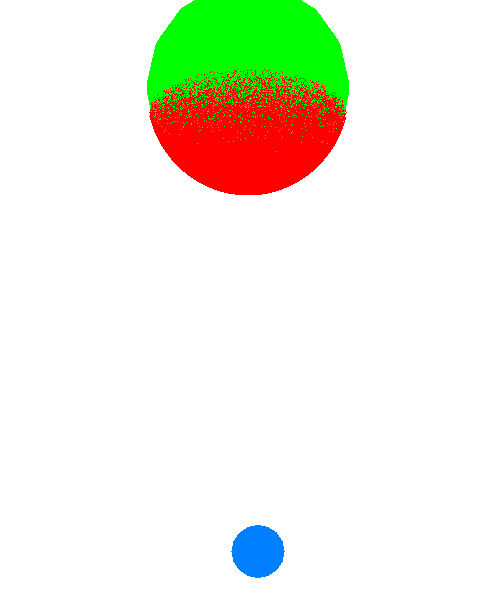
\includegraphics[width =1.0 in]{sphere_emitter.png}	}
  \caption{
Blue spherical emitter at $(0, 0, 0)$. 
Green absorber at $(0, 4, 0)$. 
Ray-sphere intersection locations are coloured in red.
A relatively low number of the photons emitted are absorbed.
Note that the interaction strength is isotropic.
}
\end{figure}


\begin{figure} 
\centering
\frame{  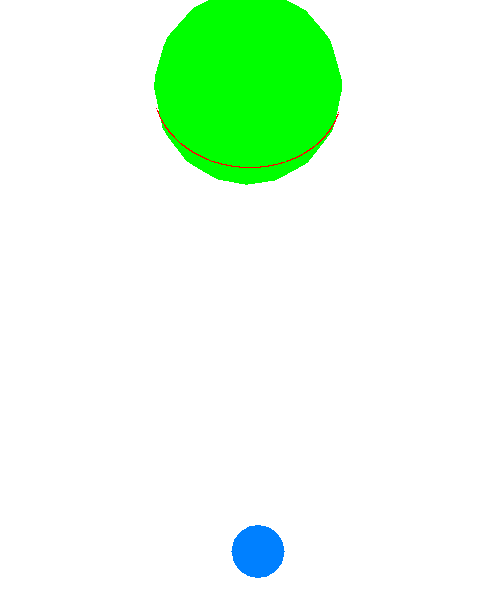
\includegraphics[width = 1.0 in]{circle_emitter.png}	}
  \caption{
Blue circular emitter at $(0, 0, 0)$. 
Green absorber at $(0, 4, 0)$. 
Ray-sphere intersection locations are coloured in red.
A relatively high number of the photons emitted are absorbed.
Note that the interaction strength orthogonal to the circle's plane reduces as the photon emitter goes from spherical to circular.
}
\end{figure}

\begin{figure} 
\centering
\frame{  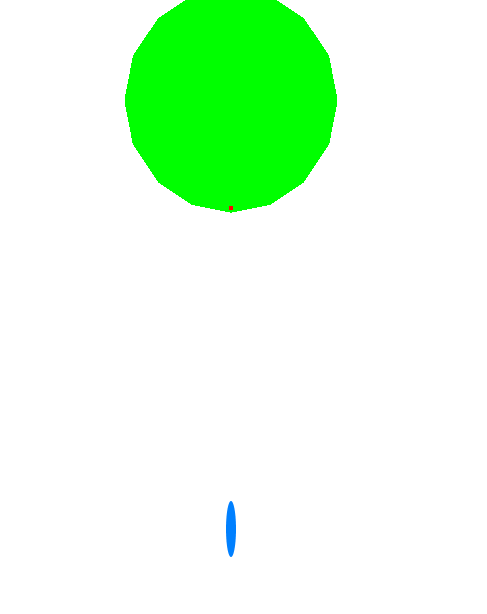
\includegraphics[width = 1.0 in]{beam_emitter.png}	}
  \caption{
Blue beam emitter at $(0, 0, 0)$. 
Green absorber at $(0, 4, 0)$. 
Ray-sphere intersection location is coloured in red.
$100\%$ of the photons emitted are absorbed.
Note that the interaction strength for all angles other than head-on reduces as the photon emitter goes from spherical to beam-like.
}
\end{figure}



\begin{figure} 
\centering
  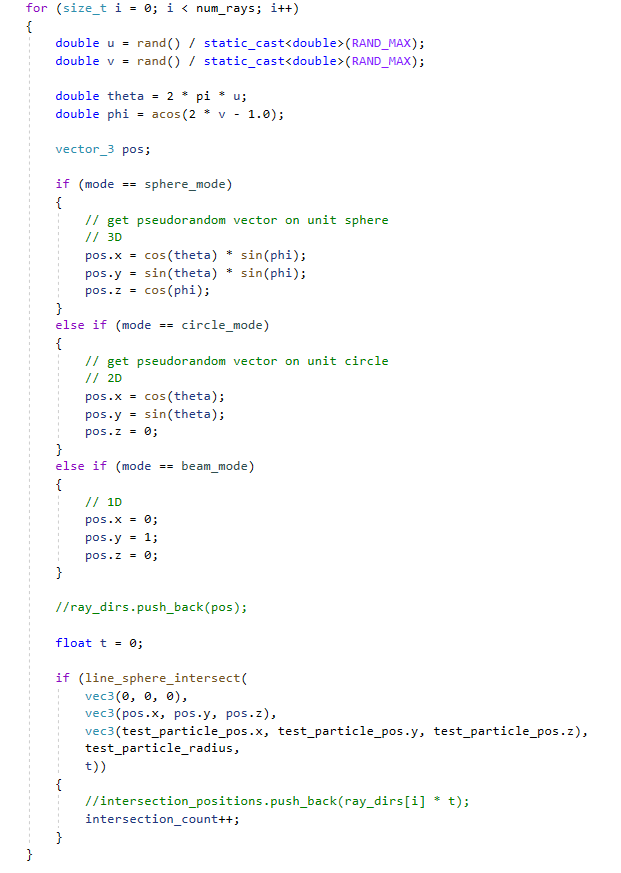
\includegraphics[width = 5 in]{code.png}	
  \caption{Normalized interaction strength $=$ intersection count $/$ number of rays.
Inverse normalized interaction strength $=$ $1.0$ $/$ normalized interaction strength.
In this paper, number of rays is $10,000,000$.
}
\end{figure}


\end{document}









